\section{A first Night Train experience}
\margininbox{Your Mum}{
     \begin{itemize}
    \item William French
    \item Tanguy Racine
    \end{itemize}}{\explo}

\subsection{Revisiting the Esoterica streamway (again)}
William had only come three days past, when I proposed to go with him down to camp. As it was proving rather crowded on the day train, we resolved to take the night train shifts. The leads close to camp were still open as far as I was concerned. I had my eye on the front of `\passage{A Pun Too Far}' in particular: it had been left unpushed since the previous year despite its relative proximity to \passage{X-Ray}. \passage{Push Your Luck} was another option.

It took a lot of convincing to depart from the Bivi when the night was young but before midnight William and I were getting changed by the entrance to \passage[cave]{Gardeners' World}. The excitement at pushing once more soon replaced any tiredness I'd felt. As I clipped into the first traverse rope, I was wide awake, conscious of every move, perhaps more than I had in the day train. I led the way down the entrance pitches, and then down to the big ones. In Pink I heard voices of exiting cavers rising from farther down. I let out a loud `Eh Oh!'

 `Eh Oh!' came the answer. Soon the lights of Jim and Dave appeared. `Eh! How's it going? Luck in your push?'.
`We went to \passage{Push Your Luck}, you and Rhys have a different conception of easy walking passage it seems and we were quite confused.' Dave explained.
`Tell me about it.'

\begin{marginfigure}
	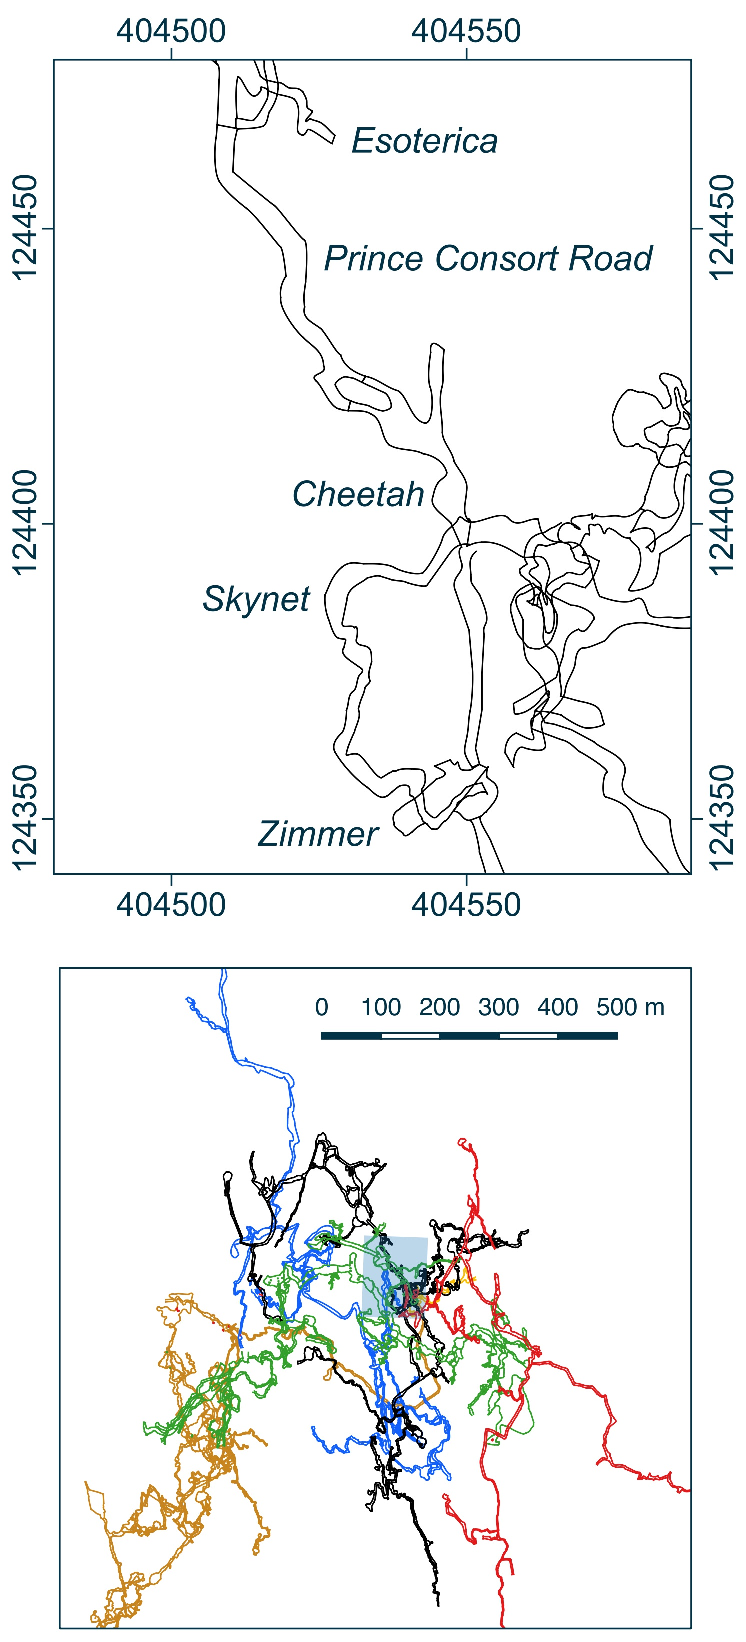
\includegraphics[width= \linewidth]{images/little_insets/esoterica_inset.pdf}
	\caption*{Plan view of \protect\passage{Prince Consort Road} and \protect\passage{Esoterica}--- Slovenian National Grid EPSG 3794}
	\label{Prince Consort Road}
\end{marginfigure}

`Well for a start we didn't find the end PSS's. We surveyed from a waterfall where we couldn't go up anymore, then took the high level to the roof until we dropped into the streamway again. There we found \passage{Push Your Luck} STN 39 and the compass broke down. We tied in there but we couldn't survey the passage from the end of \passage{Cuckoo's Nest} to STN 39.'
`Is it the very high level passage, the dry crawl?' I asked.
`It's all that same dry crawl yes, there is a chamber before we dropped back into the stream, there might be leads off it'.
`I think I understand, Rhys and I probably didn't go ALL the way up to the roof to gain the entry to the crawl from \passage{Cuckoo's Nest}. We surveyed the bottom of the rift. What did you call it?'
`\passage{Agartha}!'
`Ah, the mythical subterranean kingdoms! \passage{Mig} isn't a myth though...'.

\mydelimiter

It seemed like the easy lead at the end of \passage{Push Your Luck} was out of order so I proposed that William and I push the \passage{Esoterica} streamway. In 2014, an additional pitch had been rigged by James O'Hanlon and himself. William approved and we carried on downwards, wishing the others good speed and fair winds.

From \passage{Zimmer}, the way to \passage{Esoterica}, via \passage{Prince Consort Road} was plain sailing. At the lead I checked my watch: `4.00am'. I wedged myself into the muddy rift, rerigging with a tape the backup. From then it was a smooth descent into a small pitch, followed by a traverse on top of chockstones, wedged into a particularly narrow part of the passage, leading to the second pitch. I abseiled next to the waterfall, reached a rebelay and descended once more. The water pooled at the bottom, before escaping from a small aperture in the centre of the large bowl. To the side, the take off for \passage{Your Mum} pitch awaited.

At the bottom of the last pitch, the water ran its course to a gash in the northern wall. The lead was a narrow opening, water splashing and spraying in all directions. There seemed to be a continuation at the very bottom, in a small pit where the water gathered before disappearing from sight. \bignote{Mustering all the will to explore I could, I spidered my way down in seconds, kneeled to have a look underneath the lip of rock and proclaimed the lead dead}. Without further ado, I climbed my way up as fast as I could, cursing the curiosity that got me wet. At the top, I discouraged William to have a look, instead I dropped the end of the tape over the pit, measured it to be about 7 metres deep and recorded it in the notebook.

I looked at the watch again when we emerged in \passage{Prince Consort Road}. `5.20am'. I sat on the sandy floor, shivering. My legs were still damp from the ascending in the proximity of the waterfalls. William confirmed the water levels were quite high compared with the previous year. The passage was ever so slightly draughty and the water had slowly found its way to my skin. I grabbed a handful of sand and rubbed it on my forearms and shoulders hoping it would help the drying process. The movement got me warmer at least, so I carried on until blood was flowing all around.

I knew it was still too early to come back to \passage{X-Ray} despite William's assertion that anywhere between a half-and hour to an hour early was acceptable, and that anyway the pairs still sleeping at camp should make us dinner! Still, it was very early. Being on \passage{Prince Consort Road} it seemed a pity not to stop by the \passage{Albert Hall}, which was found very quickly past a boulder collapse. An enormous void space, with footsteps leading up a boulder field. \bignote{I was humbled by the large dimensions of the blocks, and sketched out by their lack of obvious support}.

Back at \passage{Zimmer} we were quite damp, tired and not very warm. We used \passage[mini-camp]{Gamma-Ray}'s foil blankets to keep hypothermia at bay until it was nearer 8:00am. Underneath the blanket I left my light on, and closed my eyes, lying down on a tackle sack, with a bundle of rope for pillow. At quarter to, William couldn't bear it any longer and stomped down \passage{Friendship Gallery} to wake the day train, while I emerged from the half-sleep I'd got.

Eyes still half closed, I kept my light to its lowest setting and wandered towards \passage{X-Ray}, stumbling over the now greasy boulders lining the floor. William started cooking food, while the faces of Rhys and Ben appeared one by one from the tent. Oli and Clare had slowly shifted from the night train to the day train. After several hints, Rhys and Ben started to get changed for their own pushing trip to \passage{Sic Semper Tyrannis}. I collapsed on the bed in my undersuit. I knew I had to wait a little for it to dry so I opened the logbook and started reading what had happened in my absence. Eventually I snuggled inside one of the Nitestars and fell asleep within minutes.

I woke up at three in the afternoon, but managed to fall asleep again. Only William's soft breathing interrupted the low, deep rumble of \passage{Zimmer}. We were alone in the tent since Oli and Clare had departed for the surface, after deciding not to go pushing `\passage{A Pun Too Far}'. Their trip seemed to have been a cracking one, with several hundreds of metres of passage found off \passage{Meridian Way} in either direction. Rhys and fresher Ben were pushing in the same region, far to the south.

\name{Tanguy Racine}

\subsection{More misery in a flooded streamway}
\margininbox{A Pun Too Far}{
     \begin{itemize}
    \item William French
    \item Tanguy Racine
    \end{itemize}}{\explo}
I longed for a trip close to camp that didn't involve getting drenched through waterfalls. \passage{A Pun Too Far} seemed a good option, though the lead was in a streamway. That statement doesn't make any reasonable sense: depth, isolation, tiredness and hopes of glory are the best drivers for irrational decisions. We knew we were in the middle of an apocalyptic rainstorm and we'd seen first hand its effects on the \passage{Esoterica} streamway. Why persist?

\begin{marginfigure}
	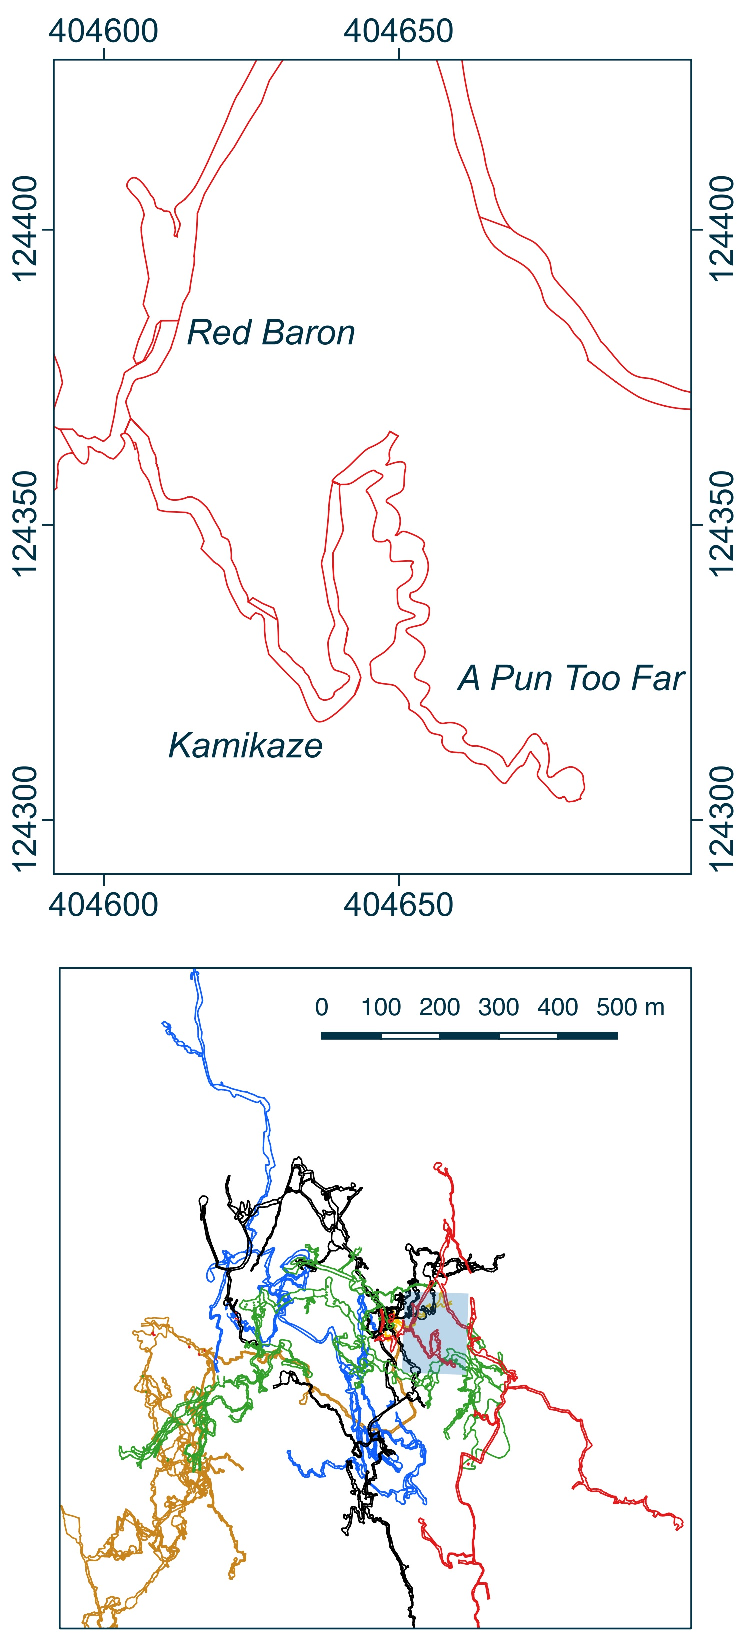
\includegraphics[width= \linewidth]{images/little_insets/pun_too_far_inset.pdf}
	\caption*{Plan view of \protect\passage{A Pun Too Far} streamway --- Slovenian National Grid EPSG 3794}
	\label{Pun too Far}
\end{marginfigure}


It was also a perfectly good lead, with plenty of depth potential, no obvious sign of closing down and a sizeable amount of water flowing through. It was also my first proper lead: I alone during the expedition knew how to get to it, negotiate the tight sections and the awkward pitch heads. So that was decided: we would go back to \passage{A Pun Too Far}. 

Unfortunately, this trip was dogged with bad luck. We arrived at the \passage{Kamikaze} crawl all right, then started the slither to the big squeeze past the boulder at the end, got through and started rerigging the three pitches of \passage{A Pun Too Far}. Once we got to the pushing front however, it became clear that there was a lot more water than in 2014, and that the levels were rising. One of the down-climbs had to be rigged to be passable, which slowed us down a little.

We quickly put some bolts in and I descended onto a spray lashed alcove: the water disappeared in a narrow crack under the far wall, while some narrow, muddy looking squeeze, quite in keeping with the spirit of the cave so far beckoned. I cursed our ill fated trip, and in a fit of anger at the cave, decided that I'd had enough and turned around. I was wet again, tired and irritable. 

Little did I know at the time that more trouble was on its way, as meanwhile on the surface, my tent was being battered by the apocalyptic weather...

\name{Tanguy Racine}
